\chapter{Deskripsi Sistem}
\label{chap:deskripsi-sistem}

\section{Deskripsi Solusi}
\label{sec:deskripsi-solusi}

Sistem pemantauan detak jantung berbasis IoT pada umumnya mengirimkan sinyal mentah secara langsung ke server \textit{cloud} untuk diproses~\cite{al_quayed_2026}. Pendekatan terpusat ini menimbulkan latensi yang tinggi, beban komputasi yang menumpuk pada server, serta ketergantungan besar terhadap kestabilan koneksi internet, sehingga sistem rentan kehilangan data ketika jaringan terganggu~\cite{resilient_edge_cloud}. Padahal, pemantauan kardiovaskular bersifat kontinu dan kritis terhadap waktu, sehingga keterlambatan maupun terputusnya aliran data dapat mengurangi efektivitas deteksi dini aritmia.

Solusi yang ditawarkan pada penelitian ini adalah sistem pemantauan detak jantung kontinu yang melakukan deteksi dini aritmia secara langsung pada mikrokontroler (\textit{on-device inference}) dengan pendekatan \textit{edge computing}, serta didukung oleh \textit{pipeline edge-to-cloud} yang tahan terhadap gangguan koneksi. Dengan memindahkan proses inferensi ke perangkat, sistem tidak lagi bergantung sepenuhnya pada \textit{cloud} untuk mengambil keputusan.

Terdapat tiga fitur utama yang menjadi klaim orisinalitas solusi ini. Pertama, preprocessing sinyal ECG dilakukan secara \textit{real-time} di perangkat menggunakan filter Butterworth dan algoritma Pan-Tompkins. Kedua, inferensi aritmia dilakukan langsung di perangkat melalui model jaringan saraf konvolusional (CNN) yang dikuantisasi ke INT8 agar ringan dijalankan pada ESP32-S3. Ketiga, \textit{pipeline edge-to-cloud} dirancang resilien dengan mekanisme \textit{buffering} lokal dan protokol MQTT untuk menjaga kontinuitas serta keutuhan data.

Ketiga fitur tersebut secara langsung menjawab permasalahan yang diuraikan pada Bab 1. Pemrosesan dan inferensi di sisi \textit{edge} menekan latensi serta mengurangi ketergantungan pada \textit{cloud}, sementara \textit{pipeline} yang resilien menjamin data tetap tersimpan dan terkirim utuh meskipun koneksi sempat terputus. Dengan demikian, sistem mampu menyediakan pemantauan aritmia yang efektif.

\section{Desain Sistem}
\label{sec:desain-sistem}

Desain sistem merupakan penjelasan teknis dari solusi yang berisi urutan proses untuk menyelesaikan permasalahan. Gambar~\ref{fig:arsitektur-sistem} menunjukkan arsitektur sistem secara \textit{high-level view} yang tersusun atas tiga lapisan, yaitu perangkat \textit{edge}, jaringan, dan \textit{cloud}.

\begin{figure}[H]
  \centering
  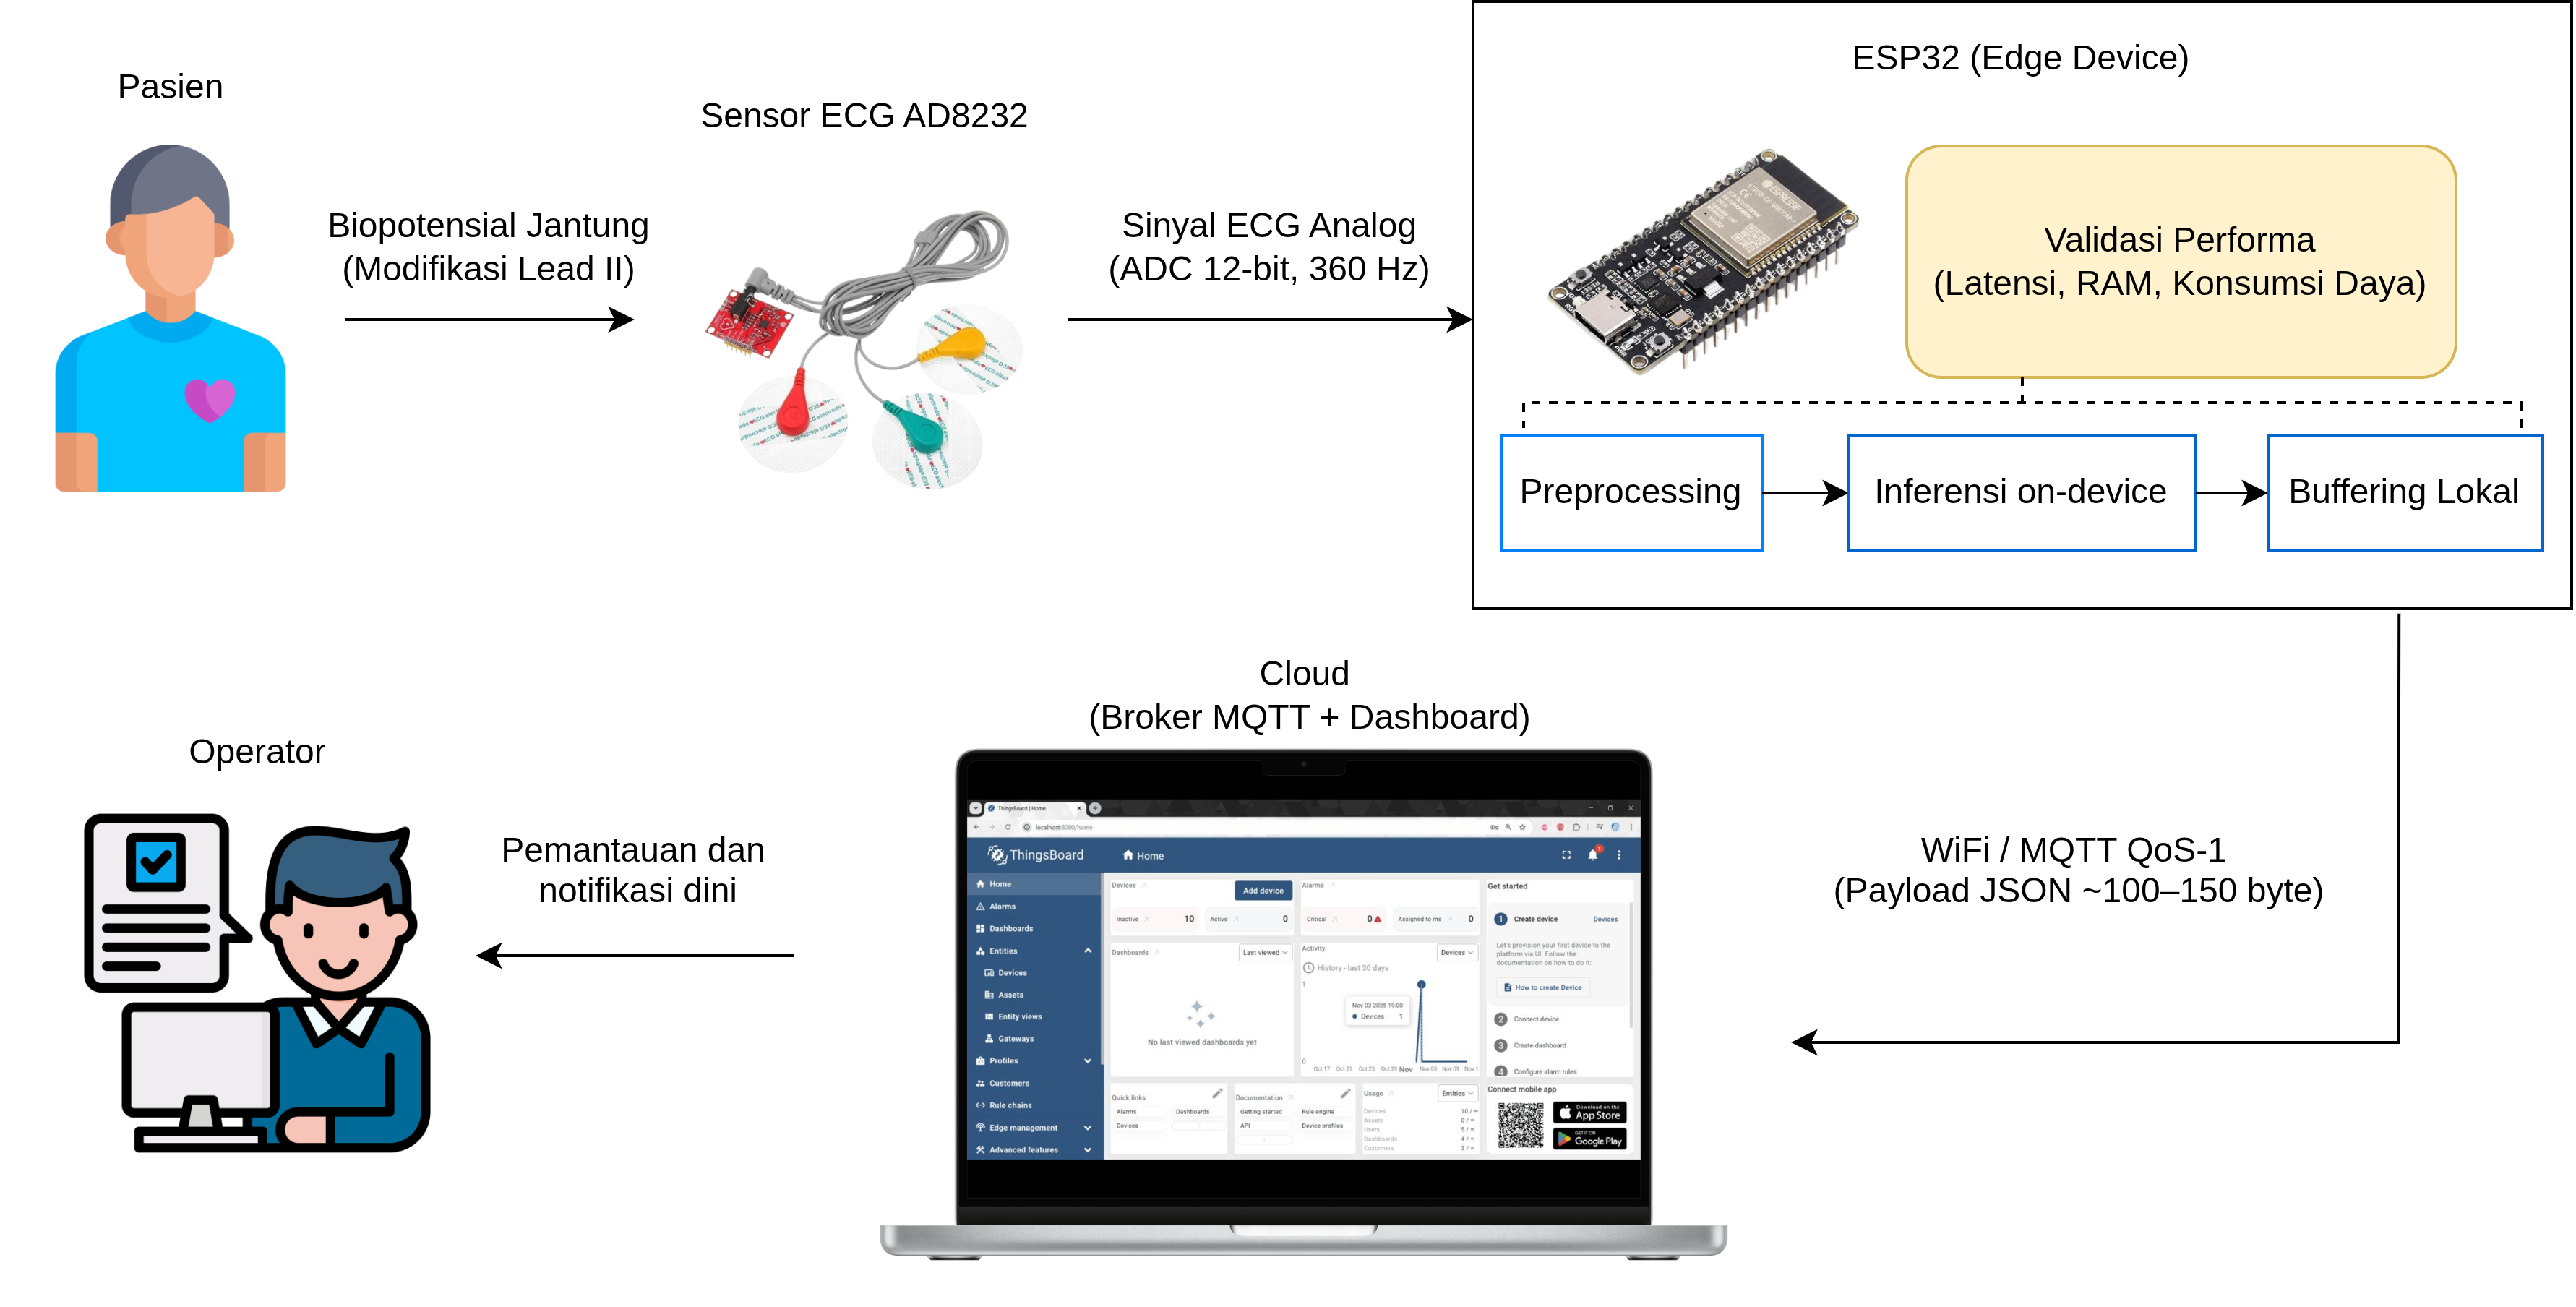
\includegraphics[width=\linewidth,keepaspectratio]{gambar/gambar_3_1.png}
  \caption{Arsitektur sistem secara \textit{high-level view}}
  \label{fig:arsitektur-sistem}
\end{figure}

Gambar~\ref{fig:arsitektur-sistem} menunjukkan bahwa sinyal ECG diakuisisi oleh sensor ECG single-lead lalu diproses sepenuhnya pada perangkat \textit{edge} berbasis ESP32-S3, mencakup preprocessing dan inferensi serta bufer data dan komunikasi MQTT. Hasil deteksi dikirim melalui jaringan WiFi menuju \textit{broker} MQTT di \textit{cloud} untuk ditampilkan pada \textit{dashboard} dan memicu notifikasi dini. Validasi performa perangkat keras dilakukan pada lapisan \textit{edge} terhadap proses preprocessing hingga inferensi. Uraian rinci tiap komponen dijelaskan pada sub-bagian berikut.

\subsection{Akuisisi dan Preprocessing Sinyal ECG}
\label{subsec:preprocessing-ecg}

Bagian ini mencakup keseluruhan proses dari pengambilan sinyal ECG hingga sinyal siap diklasifikasi oleh model. Gambar~\ref{fig:alir-preprocessing} menunjukkan flowchart preprocessing pada perangkat.

\begin{figure}[H]
  \centering
  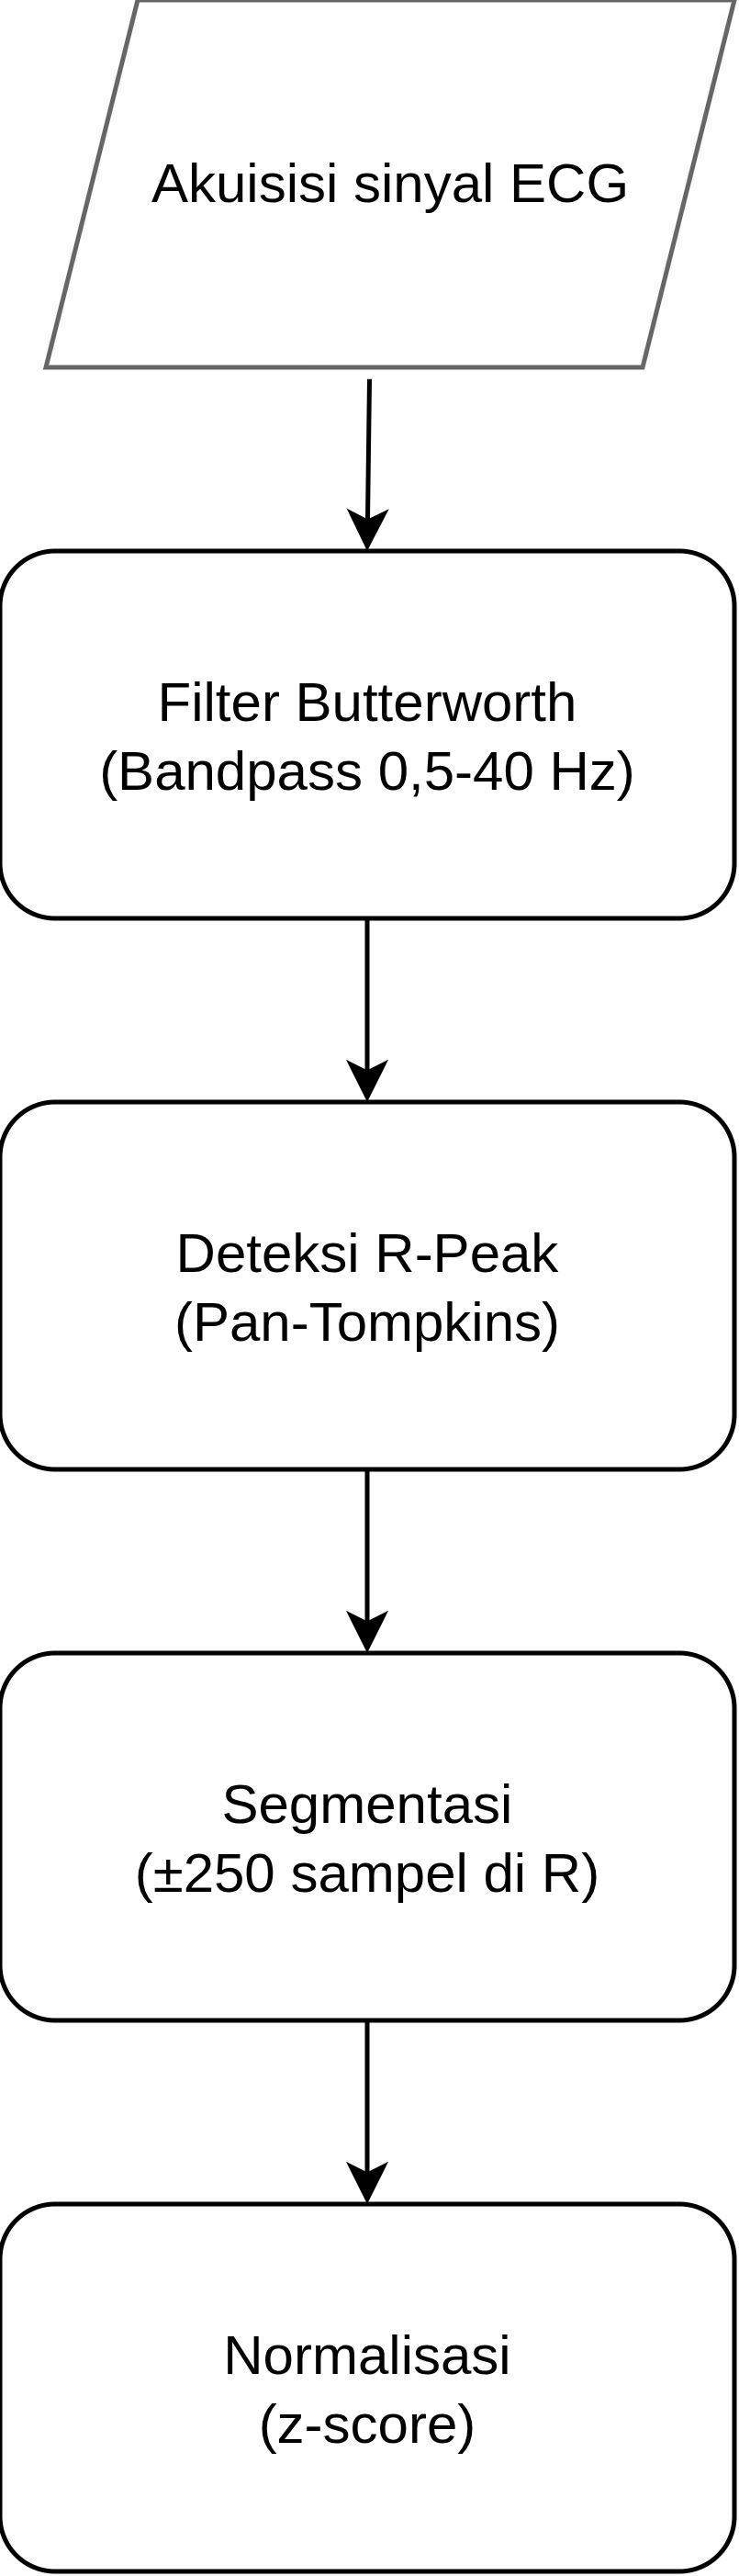
\includegraphics[height=0.6\textheight,keepaspectratio]{gambar/gambar_3_2.png}
  \caption{Flowchart preprocessing pada perangkat}
  \label{fig:alir-preprocessing}
\end{figure}

\subsubsection{Akuisisi Sinyal ECG}

Sinyal ECG diperoleh menggunakan modul sensor AD8232 yang dikonfigurasi pada Lead II. Lead II dipilih karena vektor listrik jantung sejajar dengan sudut pandang sadapan tersebut sehingga gelombang R muncul paling tinggi dan tegak, menjadikannya paling andal untuk analisis irama~\cite{ecg_goldberger}. Konfigurasi single-lead ini memadai untuk deteksi aritmia sekaligus selaras dengan rekaman yang dipakai pada \textit{dataset}, yaitu \textit{Modified Lead II} yang dikenal sebagai MLII. Sinyal analog kemudian disampel oleh ADC (\textit{Analog-to-Digital Converter}) pada ESP32-S3, dengan laju sampel disesuaikan terhadap \textit{dataset} acuan, yaitu 360 Hz.

\subsubsection{Filter Butterworth}

Sinyal ECG mentah mengandung \textit{noise} berupa pergeseran garis dasar (\textit{baseline wander}) pada frekuensi rendah serta \textit{noise} otot dan interferensi listrik pada frekuensi tinggi. Filter Butterworth \textit{bandpass} dengan frekuensi \textit{cutoff} 0,5--40 Hz digunakan untuk membuang kedua jenis \textit{noise} tersebut sambil mempertahankan pita ECG yang berguna~\cite{sornmo_laguna_2005}. Filter berorde 2--4 dinilai memadai dan diimplementasikan sebagai \textit{second-order section} (\textit{biquad}) yang bersifat kausal, sehingga ringan secara komputasi dan dapat diproses sampel demi sampel secara \textit{real-time} pada mikrokontroler.

\subsubsection{Deteksi R-peak dengan Algoritma Pan-Tompkins}

Algoritma Pan-Tompkins digunakan untuk menentukan lokasi R-\textit{peak} pada sinyal yang telah bersih. Algoritma ini menonjolkan energi kompleks QRS melalui rangkaian tahapan, yaitu \textit{bandpass} filter 5--15 Hz, turunan, pengkuadratan, integrasi jendela bergerak, serta \textit{threshold} adaptif dengan periode refraktori~\cite{pan_tompkins_1985}. Keluaran algoritma berupa lokasi R-\textit{peak} yang selanjutnya menjadi titik acuan segmentasi.

\subsubsection{Segmentasi dan Normalisasi}

Berdasarkan setiap lokasi R-\textit{peak}, sinyal dipotong menjadi \textit{window} berukuran tetap sepanjang 250 sampel, yaitu 90 sampel sebelum dan 160 sampel sesudah R-\textit{peak}, sehingga gelombang P di awal dan gelombang T di akhir detak ikut terekam. Gambar~\ref{fig:segmentasi} mengilustrasikan proses segmentasi berbasis R-peak beserta
efek normalisasi z-score.

\begin{figure}[H]
  \centering
  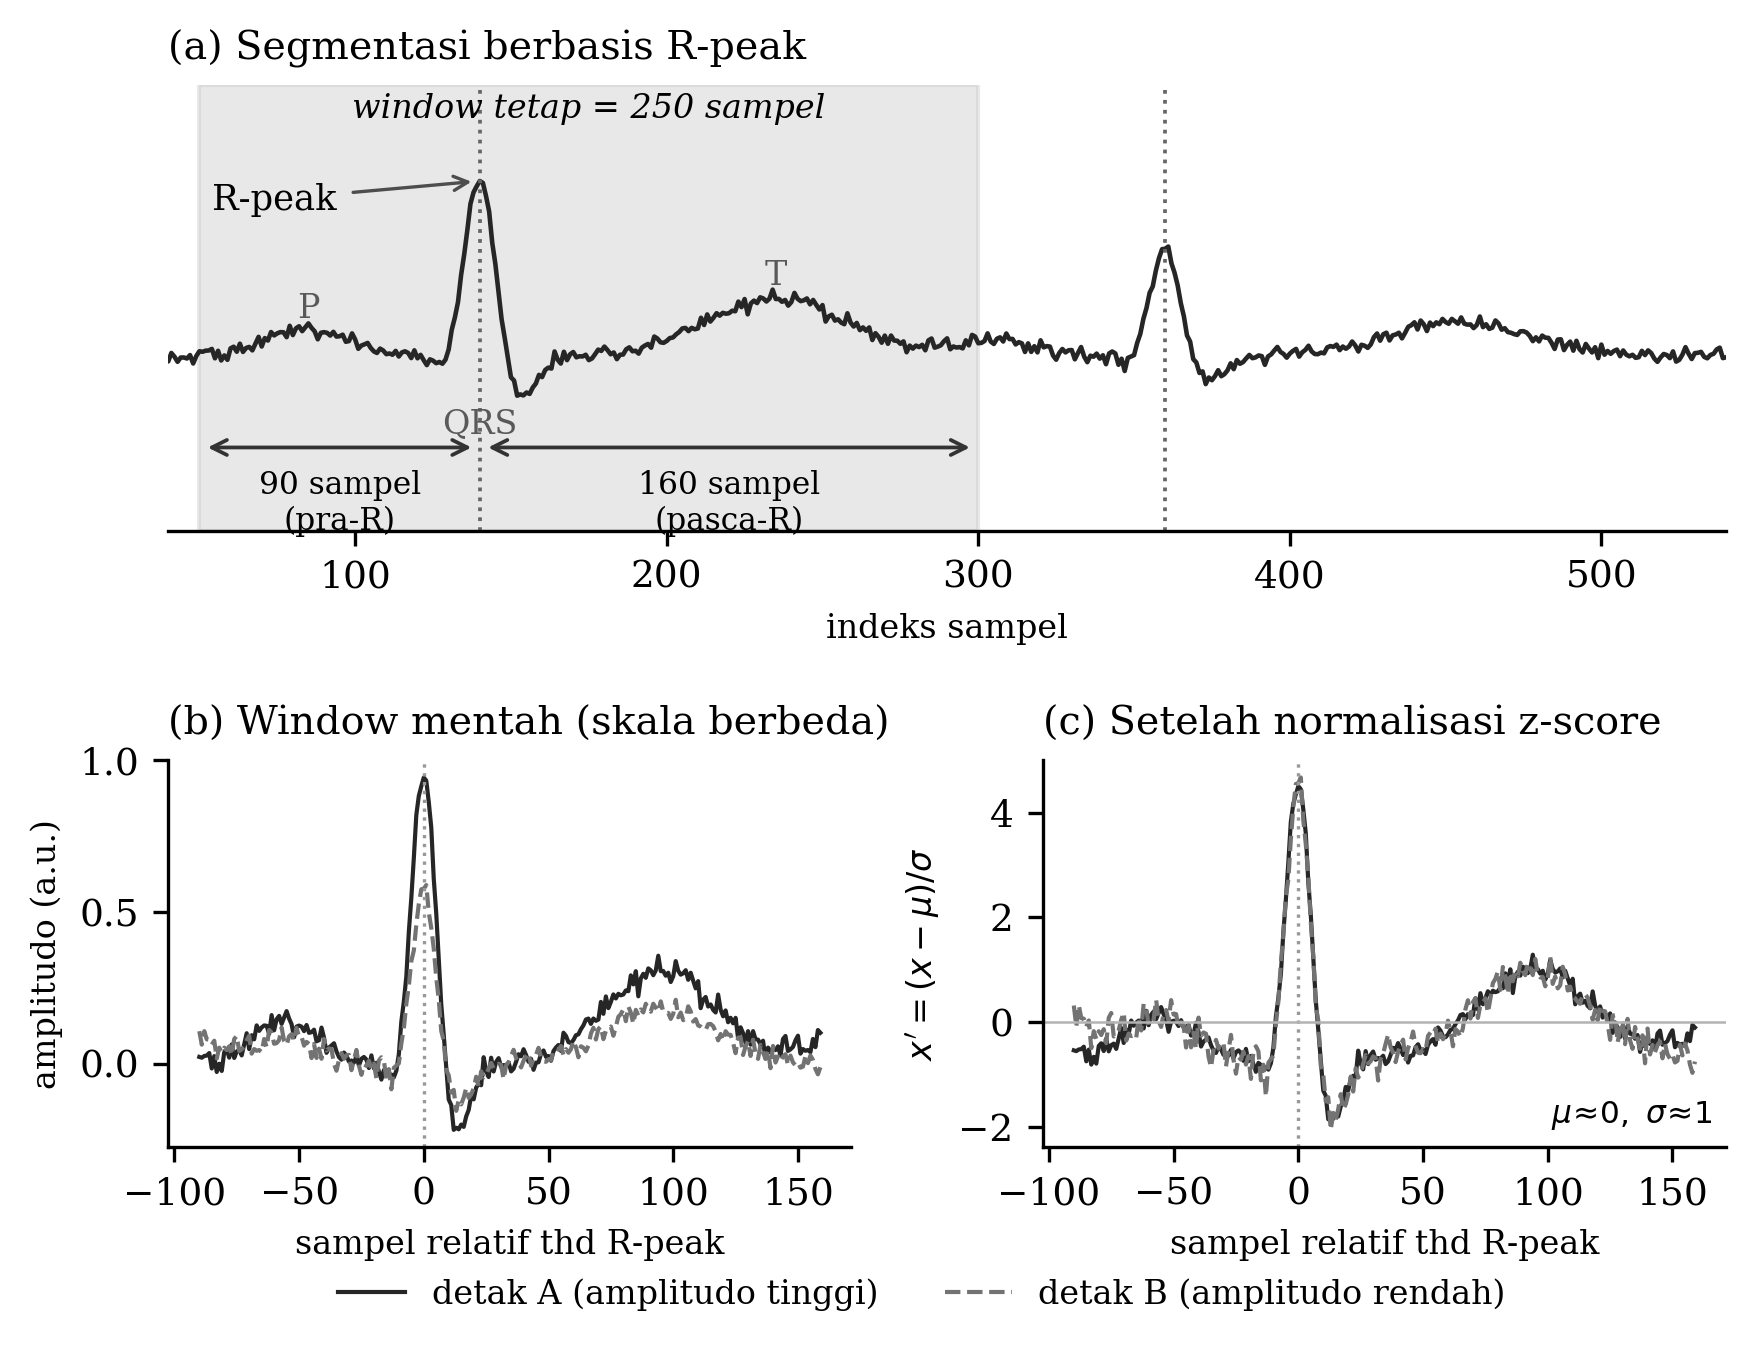
\includegraphics[width=0.9\linewidth]{gambar/gambar_segmentasi_normalisasi.png}
  \caption{Ilustrasi segmentasi berbasis R-peak dan efek normalisasi z-score}
  \label{fig:segmentasi}
\end{figure}

Setiap \textit{window} selanjutnya dinormalisasi menggunakan \textit{z-score} sebagaimana ditunjukkan pada Persamaan~\ref{eq:normalisasi}, agar model berfokus pada bentuk sinyal dan tidak terpengaruh oleh perbedaan amplitudo antarperangkat maupun antarpasien.

\begin{equation}
\label{eq:normalisasi}
x' = \frac{x-\mu}{\sigma}
\end{equation}

Persamaan~\ref{eq:normalisasi} menunjukkan proses normalisasi, dengan $x$ adalah nilai sampel, $\mu$ adalah rata-rata \textit{window}, dan $\sigma$ adalah simpangan baku \textit{window}. Penambahan konstanta kecil pada penyebut dilakukan untuk menghindari pembagian dengan nol.

\subsection{Model Klasifikasi Aritmia}
\label{subsec:model-tinyml}

Bagian ini menguraikan model yang digunakan untuk mengklasifikasikan setiap detak, mulai dari penyiapan data, arsitektur model, hingga proses pelatihan dan kuantisasi.

\subsubsection{Dataset dan Pelabelan}

Dataset yang digunakan adalah MIT-BIH \textit{Arrhythmia Database}, yang terdiri atas 48 rekaman berdurasi sekitar 30 menit, tersampel pada 360 Hz, dengan kanal rekaman utama berupa modifikasi sadapan Lead II (MLII) dan anotasi per-detak oleh kardiolog~\cite{moody_mark_2001}. Tugas klasifikasi dirumuskan secara biner, yaitu Normal dan Aritmia, sejalan dengan tujuan deteksi dini. Skema anotasi AAMI sebenarnya memungkinkan klasifikasi multi-kelas (N, S, V, F, Q), namun skema ini tidak diadopsi pada penelitian ini karena distribusi kelas F dan Q pada MIT-BIH sangat timpang antarpasien. Pada skema pembagian \textit{inter-patient} (DS1/DS2), sejumlah rekaman bahkan tidak memiliki representasi kedua kelas tersebut sama sekali, sehingga metrik evaluasi untuk kelas minoritas ini berpotensi tidak stabil dan tidak representatif. Klasifikasi biner dipilih agar evaluasi model tetap dapat diandalkan pada seluruh partisi data, sejalan dengan peran sistem sebagai \textit{early warning} yang membedakan kondisi normal dari kondisi yang memerlukan perhatian lanjut, tanpa mengklaim kemampuan diagnosis diferensial antarjenis aritmia. Pemetaan simbol anotasi MIT-BIH menjadi label biner ditunjukkan pada Tabel~\ref{tab:pemetaan-label}.

\begin{table}[!ht]
  \centering
  \caption{Pemetaan simbol anotasi MIT-BIH menjadi label biner}
  \label{tab:pemetaan-label}
  \begin{tabular}{|c|l|c|}
    \hline
    \rowcolor{headgray}
    \textbf{Simbol Anotasi} & \textbf{Jenis Detak} & \textbf{Label Biner} \\
    \hline
    N & Detak sinus normal & Normal \\
    \hline
    V & Kontraksi ventrikular prematur & Aritmia \\
    \hline
    S & Detak supraventrikular & Aritmia \\
    \hline
    F & Detak fusi & Aritmia \\
    \hline
    Q & Detak tidak tergolong & Aritmia \\
    \hline
  \end{tabular}
\end{table}

Tabel~\ref{tab:pemetaan-label} menunjukkan bahwa hanya detak sinus normal yang dikategorikan sebagai Normal, sedangkan seluruh detak menyimpang dikategorikan sebagai Aritmia. Penggolongan beberapa kelainan konduksi mengikuti standar yang akan dikonfirmasi lebih lanjut pada pelaksanaan eksperimen.

% ============================================================
% ARSIP (dinonaktifkan sementara) --- Validasi cross-database INCART & SVDB
% Alasan: pembandingan dengan dataset selain MIT-BIH masih menunggu
%         pertimbangan lebih lanjut. Teks tidak dihapus, hanya diarsipkan.
% Cara aktifkan lagi: hapus baris \iffalse dan \fi pembungkus di bawah.
% Dokumentasi: proposal-pa/docs/arsip-cross-dataset.md
% ============================================================
\iffalse
Untuk menguji generalisasi model secara lebih menyeluruh, selain MIT-BIH Arrhythmia
Database sebagai dataset utama (pelatihan DS1 dan pengujian DS2 secara antarpasien),
penelitian ini juga merencanakan validasi \emph{cross-database}
menggunakan dua basis data pelengkap~\cite{goldberger_2000_physionet}. Pertama, St.
Petersburg INCART 12-lead Arrhythmia Database yang memuat proporsi detak ventrikular
jauh lebih besar sehingga menguji ketahanan deteksi kelas ventrikular pada kondisi
akuisisi yang berbeda. Kedua, MIT-BIH Supraventricular Arrhythmia Database (SVDB) yang
secara khusus memperkaya sampel detak supraventrikular (kelas S), sehingga menjadi
pengujian langsung terhadap efektivitas cabang ritme yang dirancang untuk membedakan
detak supraventrikular. Ketiga basis data memiliki frekuensi sampling yang berbeda
(MIT-BIH 360 Hz, INCART 257 Hz, SVDB 128 Hz), sehingga seluruh rekaman terlebih dahulu
diselaraskan (\emph{resample}) ke frekuensi seragam 360 Hz agar konsisten dengan ukuran
\emph{window} 250 sampel dan pipeline Pan-Tompkins. Pemetaan anotasi mengikuti standar
AAMI yang sama pada ketiga basis data sehingga skema klasifikasi biner tetap berlaku.
\fi

Selain segmen \textit{window} 250 sampel, pada tahap penyiapan data juga dihitung fitur interval RR per-detak berupa RR\_prev, rasio RR, dan $\Delta$RR dari lokasi R-\textit{peak} keluaran algoritma Pan-Tompkins, untuk menjadi masukan cabang ritme pada model.

\subsubsection{Perancangan Arsitektur Model}

Pola umum perancangan model CNN untuk klasifikasi sinyal ECG pada perangkat
\textit{embedded} telah divalidasi oleh beberapa penelitian sebelumnya. Mekhfioui et
al.~\cite{mekhfioui_2025} mengusulkan arsitektur 1D-CNN dengan tiga blok Conv1D
bertingkat, Global Average Pooling (GAP) sebagai pengganti lapisan \emph{flatten}, dan
lapisan sigmoid untuk klasifikasi biner. Pola morfologi inilah yang diadopsi sebagai
cabang morfologi pada penelitian ini, dengan penyesuaian jumlah \emph{filter}
(16/32/32) agar lebih ringan dan sesuai batasan SRAM (\textit{Static RAM}) ESP32-S3. Kelayakan menjalankan
model sejenis secara \emph{on-device} dalam format INT8 pada mikrokontroler ditunjukkan
oleh Kim et al.~\cite{kim_2023} melalui TinyCES (ukuran 27 KB pada Cortex-M4).
Lebih jauh, Zambrano-de la Torre et al.~\cite{zambrano_2026} membuktikan bahwa pipeline
yang hampir identik dengan penelitian ini dapat berjalan bahkan pada Arduino UNO 8-bit
yang jauh lebih terbatas daripada ESP32-S3.

Gambar~\ref{fig:pipeline-training} menunjukkan arsitektur model \textit{hybrid} yang diusulkan, terdiri atas cabang morfologi dan cabang ritme.

\begin{figure}[H]
  \centering
  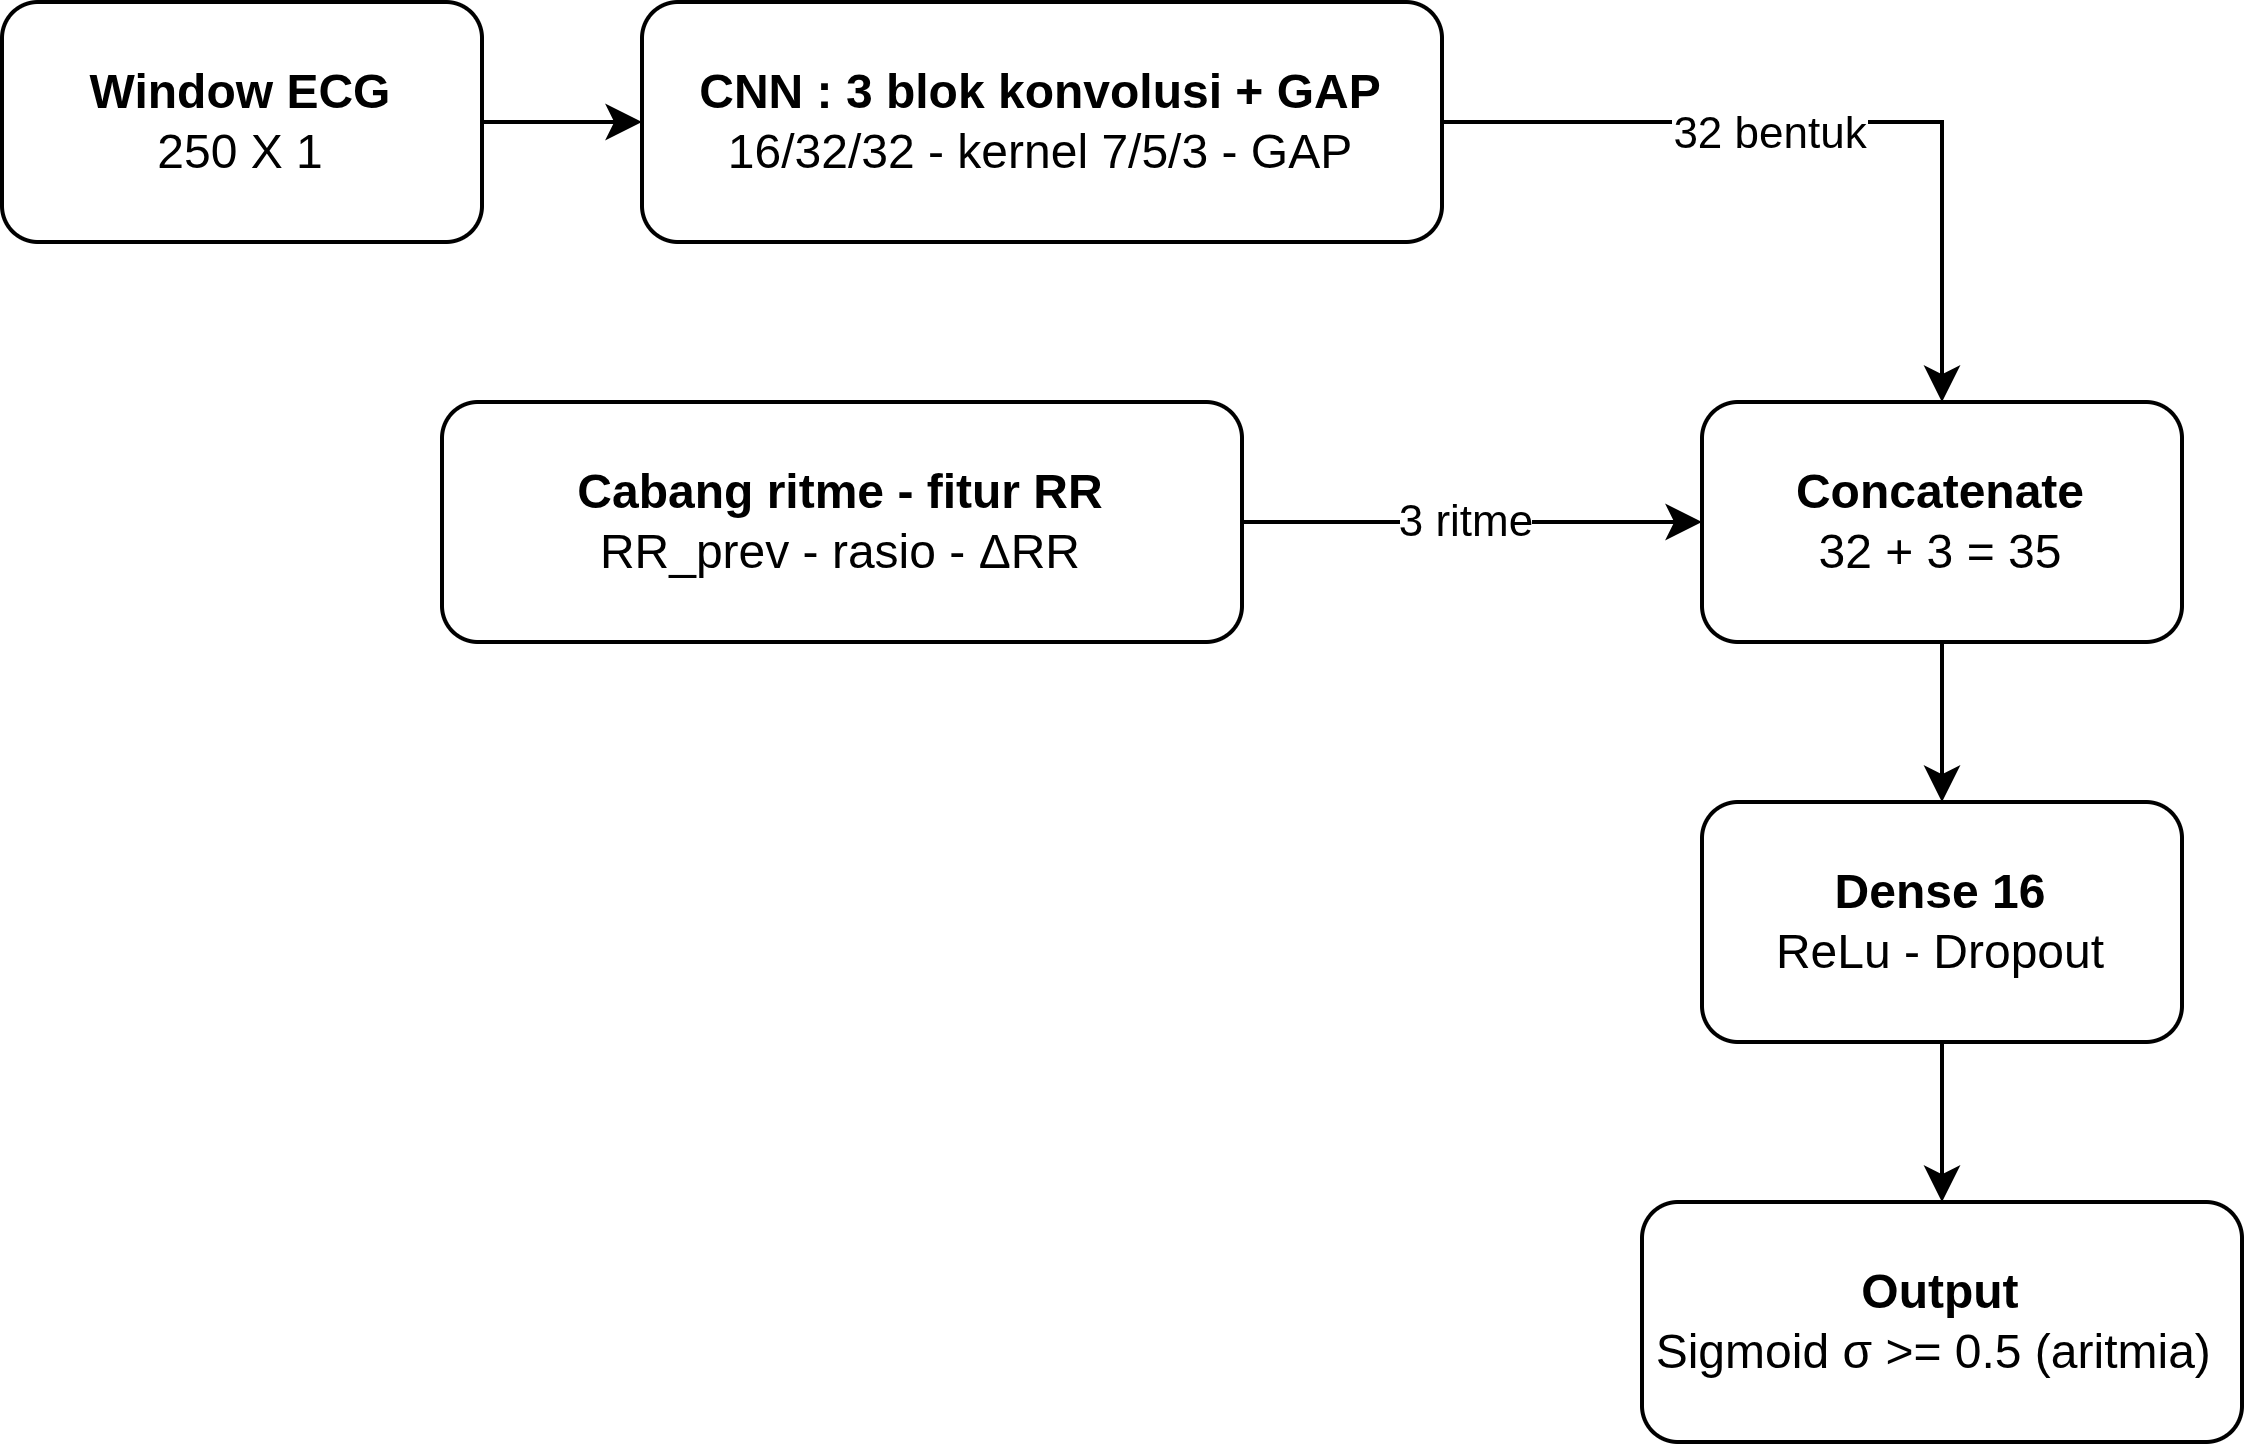
\includegraphics[width=0.92\linewidth,keepaspectratio]{gambar/gambar_3_4.png}
  \caption{Arsitektur model CNN \textit{hybrid} dengan fitur RR}
  \label{fig:pipeline-training}
\end{figure}

Model yang diusulkan berbentuk arsitektur \textit{hybrid} dua cabang. Cabang
pertama, yaitu cabang morfologi, adalah jaringan saraf konvolusional
(\textit{Convolutional Neural Network}, CNN) ringkas yang bekerja langsung
pada \textit{window} ECG 250 sampel, terdiri atas tiga blok konvolusi dengan
16, 32, dan 32 \textit{filter} serta ukuran \textit{kernel} 7, 5, dan 3, yang
masing-masing diikuti aktivasi ReLU dan \textit{max-pooling}. Lapisan-lapisan
tersebut kemudian diringkas oleh \textit{Global Average Pooling} menjadi 32
fitur morfologi yang merepresentasikan bentuk gelombang PQRST tiap detak.

Klasifikasi yang murni berbasis morfologi per-detak memiliki keterbatasan pada
detak supraventrikular (kelas S). Morfologi detak supraventrikular kerap
menyerupai detak normal, sehingga pembeda utamanya justru terletak pada
\textit{timing} kemunculannya yang prematur, yaitu informasi yang tidak
tertangkap oleh bentuk gelombang tunggal. Untuk mengatasi keterbatasan ini,
penelitian ini menambahkan cabang kedua, yaitu cabang ritme, berupa fitur
interval R-R (RR) per-detak. Penggabungan fitur
morfologi dengan fitur interval RR merupakan pendekatan yang telah terbukti
memperbaiki deteksi kelas supraventrikular pada klasifikasi
\textit{inter-patient}~\cite{dechazal_2004}.

Fitur RR diturunkan langsung dari lokasi R-\textit{peak} keluaran algoritma
Pan-Tompkins, sehingga tidak
memerlukan komputasi tambahan yang berarti. Tiga fitur kausal digunakan agar
sistem tetap beroperasi secara \textit{real-time} tanpa perlu menunggu detak
berikutnya, yaitu RR\_prev sebagai interval ke detak sebelumnya, rasio RR
yang merupakan RR\_prev dibagi rata-rata RR berjalan untuk menangkap derajat
prematuritas detak, serta $\Delta$RR sebagai perubahan interval antardetak
berurutan. Ketiga fitur dinormalisasi terlebih dahulu agar skalanya sebanding
dengan fitur morfologi.

Kedua cabang disatukan melalui operasi \textit{concatenation} setelah
\textit{Global Average Pooling}, menghasilkan vektor gabungan berdimensi 35
yang terdiri atas 32 fitur morfologi ditambah 3 fitur ritme. Vektor gabungan
ini diteruskan ke lapisan \textit{Dense} berisi 16 neuron dengan aktivasi
ReLU dan \textit{Dropout} untuk menekan \textit{overfitting}, kemudian lapisan
keluaran dengan fungsi aktivasi \textit{sigmoid} sebagaimana
Persamaan~\ref{eq:sigmoid}.

\begin{equation}
\label{eq:sigmoid}
\hat{y} = \frac{1}{1+e^{-z}}
\end{equation}

Persamaan~\ref{eq:sigmoid} menunjukkan fungsi \textit{sigmoid} pada lapisan
keluaran, dengan $z$ adalah keluaran lapisan sebelumnya dan $\hat{y}$ adalah
peluang sebuah detak tergolong aritmia. Nilai $\hat{y} \geq 0{,}5$
diklasifikasikan sebagai Aritmia. \textit{Threshold} ini bersifat dapat dikalibrasi, dan
menurunkannya akan meningkatkan sensitivitas deteksi sesuai prioritas sistem
sebagai pendeteksi dini. Penggunaan \textit{Global Average Pooling} dipilih
untuk menekan jumlah parameter secara drastis dibandingkan perataan langsung
(\textit{flatten}), sehingga model tetap berukuran kecil dan tahan terhadap
\textit{overfitting}, sesuai pendekatan yang divalidasi oleh Mekhfioui
et al.~\cite{mekhfioui_2025}. Penambahan cabang ritme hanya menambah sedikit
parameter karena lapisan \textit{Dense} menerima 35 alih-alih 32 masukan,
sehingga total parameter model tetap sekitar enam ribu dan ukuran model
setelah kuantisasi INT8 tetap di bawah 20 KB.

\subsubsection{Pelatihan dan Kuantisasi INT8}

Model direncanakan dilatih secara \textit{offline} pada komputer, kemudian hasilnya dikuantisasi agar ringan dijalankan di perangkat. Model bersifat \textit{hybrid} dengan dua masukan yang diimplementasikan menggunakan \textit{Functional API} Keras, yaitu satu masukan berupa \textit{window} ECG untuk cabang morfologi dan satu masukan berupa vektor fitur RR ternormalisasi untuk cabang ritme. Untuk memastikan evaluasi mencerminkan kondisi nyata, pembagian data direncanakan dilakukan secara antarpasien (\textit{inter-patient}), yaitu rekaman yang dipakai untuk melatih dan menguji model berasal dari kelompok pasien yang berbeda sehingga tidak terjadi kebocoran data antarpasien. Detail konfigurasi pelatihan, penanganan ketidakseimbangan kelas, serta strategi optimasi akan ditetapkan pada tahap eksperimen.

Distribusi kelas pada MIT-BIH sangat timpang, dengan detak normal yang mendominasi
sementara detak supraventrikular sangat sedikit, sehingga penanganan ketidakseimbangan kelas
menjadi bagian penting dari pelatihan. Strategi yang direncanakan meliputi pembobotan
kelas (\emph{class weighting}) pada fungsi \emph{loss} atau penyeimbangan sampel kelas
minoritas, agar model tidak bias terhadap kelas mayoritas dan \emph{recall} kelas
aritmia tetap tinggi. Selain itu, himpunan
data representatif untuk kuantisasi pasca-pelatihan (\emph{post-training quantization})
disusun agar mencakup seluruh kelas, bukan hanya kelas normal, sehingga rentang
kuantisasi terkalibrasi dengan tepat untuk kelas langka.

Setelah dilatih, model akan dikuantisasi ke INT8 agar ukurannya jauh berkurang dan dapat dikonversi ke format TensorFlow Lite Micro untuk dijalankan pada mikrokontroler~\cite{laiu_2026}. Target ukuran model setelah kuantisasi berada di bawah 20 KB, jauh lebih kecil dari kapasitas SRAM internal ESP32-S3 sekitar 512 KB (didukung PSRAM, yaitu \textit{Pseudo-Static RAM}, berkapasitas 8 MB), sehingga model diperkirakan muat dengan tetap menyisakan ruang yang memadai untuk \textit{tensor arena} dan bufer data.

\subsection{Pipeline Edge-to-Cloud yang Resilien}
\label{subsec:pipeline-edge-cloud}

Bagian ini menjelaskan integrasi seluruh proses ke dalam alur kerja \textit{firmware} sekaligus mekanisme ketahanannya terhadap gangguan koneksi. Gambar~\ref{fig:alir-firmware} menunjukkan flowchart \textit{runtime firmware} beserta jalur penanganan kondisi daring dan luring. Berbeda dari pendekatan berbasis penyimpanan non-volatil (kartu SD atau SPIFFS), resiliensi pada penelitian ini dirancang sepenuhnya di memori volatil (PSRAM) dengan asumsi perangkat \textit{wearable} diisi daya secara rutin, sebagaimana perangkat \textit{smartwatch}. Pendekatan ini menghilangkan kompleksitas manajemen \textit{filesystem embedded} serta menekan konsumsi daya dan ruang PCB. Prinsip yang mendasari rancangan ini adalah mempertahankan kelengkapan data di sisi \textit{edge} selama gangguan berlangsung, alih-alih mengandalkan rekonstruksi data yang hilang di sisi \textit{cloud}. Strategi preventif semacam ini diutamakan karena teknik imputasi sulit memulihkan informasi yang hilang bertepatan dengan kejadian seperti deteksi aritmia~\cite{resilient_edge_cloud}.

\begin{figure}[H]
  \centering
  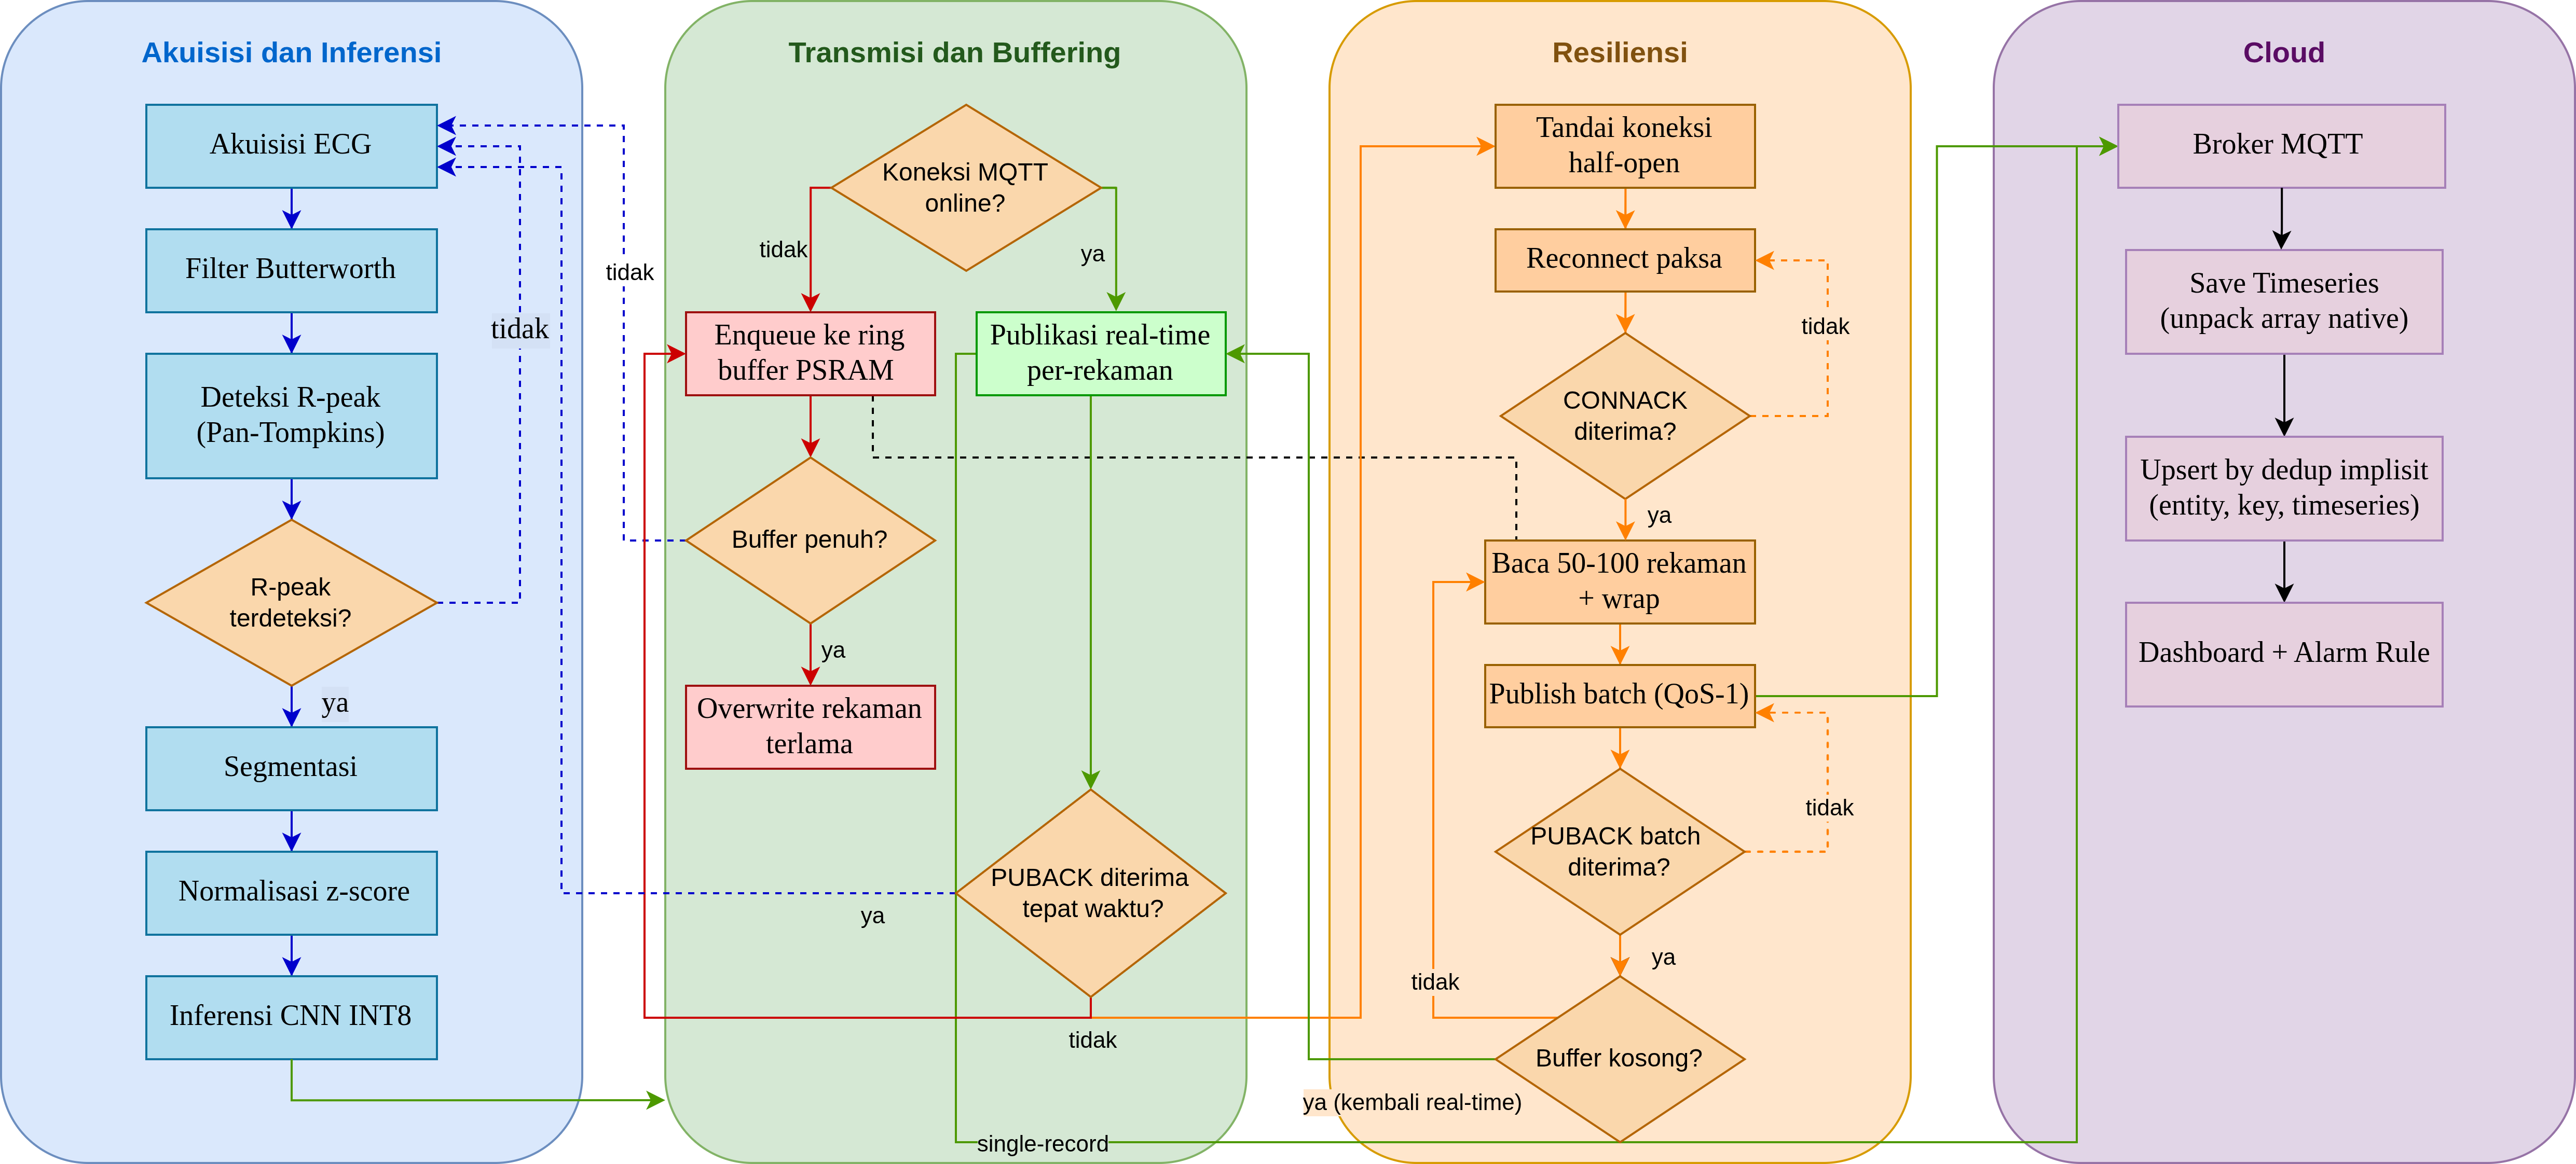
\includegraphics[width=\linewidth,keepaspectratio]{gambar/gambar_3_5.png}
  \caption{Diagram alir \textit{runtime firmware} dan jalur resilien (bufer PSRAM, \textit{batch offload}, deteksi \textit{half-open})}
  \label{fig:alir-firmware}
\end{figure}

\subsubsection{\textit{Ring Buffer} FIFO di PSRAM}

Varian ESP32-S3 yang digunakan (N16R8) memiliki PSRAM eksternal berkapasitas 8 MB
yang dapat diakses melalui fungsi heap\_caps\_malloc dengan flag MALLOC\_CAP\_SPIRAM.
Sebagian dari kapasitas ini dialokasikan sebagai partisi tetap untuk struktur data
\textit{ring buffer} (FIFO) yang menampung hasil inferensi selama koneksi jaringan
terputus, sementara sisanya tetap disediakan untuk kebutuhan lain yang turut memakai
PSRAM, yaitu \textit{tensor arena} TensorFlow Lite Micro, bufer \textit{stack} WiFi/MQTT,
dan \textit{heap} umum sistem. Dengan alokasi partisi sekitar 4 MB dan ukuran
\textit{payload} per detak $\approx$150 byte, \textit{ring buffer} mampu menampung
$\pm$27.000 rekaman, atau setara $\pm$4--7 jam pemantauan kontinu pada laju rata-rata
60--100 bpm. Kapasitas ini jauh melebihi target durasi gangguan jaringan pada skenario
pengujian pipeline, sehingga penyimpanan
non-volatil tidak diperlukan untuk memenuhi target resiliensi jaringan yang ditetapkan.

Apabila durasi gangguan jaringan melampaui kapasitas \textit{ring buffer}, mekanisme
yang diterapkan adalah \textit{overwrite} data terlama (rekaman tertua ditimpa oleh
rekaman terbaru). Mekanisme ini dipilih karena, dalam konteks pemantauan kontinu,
ketersediaan data terkini lebih relevan bagi tujuan deteksi dini dibandingkan lengkapnya
histori yang sudah kedaluwarsa. Perilaku ini dapat dikonfigurasi lebih lanjut pada tahap
implementasi sesuai kebutuhan.

\subsubsection{Transmisi \textit{Real-Time} dan \textit{Batch Offloading} saat \textit{Reconnect}}

Selama koneksi tersedia, setiap hasil inferensi langsung dipublikasikan ke broker MQTT
satu per satu (mode \textit{real-time}), sehingga \textit{dashboard} tetap memperbarui
tampilan dengan latensi minimal. \textit{Ring buffer} PSRAM hanya terisi ketika koneksi
terputus.

Ketika koneksi pulih, perangkat tidak mengirim data yang tertahan satu per satu,
melainkan merangkumnya (\textit{batching}) menjadi kelompok 50--100 rekaman per paket
dalam bentuk array JSON, mengikuti format \textit{multiple timestamped key-value pairs}
yang didukung secara native oleh ThingsBoard. Ukuran satu paket batch (50--100 $\times$
$\pm$150 byte $\approx$ 7,5--15 KB) berada jauh di bawah batas ukuran pesan MQTT pada
broker maupun jaringan WiFi lokal. Pendekatan ini mengurangi jumlah \textit{round-trip}
request-PUBACK (PUBACK adalah \textit{Publish Acknowledgement}, paket konfirmasi
penerimaan pesan oleh broker) hingga 50--100 kali lipat dibandingkan pengiriman per-rekaman, sehingga
proses \textit{flush} backlog jauh lebih cepat dan overhead jaringan turun
signifikan. Setiap paket batch tetap dikirim dengan MQTT QoS-1 (\textit{Quality of Service} tingkat 1), yaitu perangkat menunggu
konfirmasi PUBACK untuk keseluruhan batch sebelum menggeser \textit{read pointer} ke
batch berikutnya. Apabila PUBACK tidak diterima dalam tenggang waktu tertentu, batch
yang sama dikirim ulang. Setelah seluruh backlog di PSRAM terkirim dan terkonfirmasi,
perangkat kembali ke mode transmisi \textit{real-time} per-rekaman. Prinsip pemisahan
antara proses akuisisi data dan proses pengiriman data melalui bufer perantara ini
menerapkan pendekatan \textit{intermediate buffering}, karena bufer internal MQTT
(default $\pm$10 pesan \textit{in-flight}) tidak memadai untuk gangguan koneksi yang
berlangsung lebih dari beberapa detik, sehingga dibutuhkan lapisan bufer aplikasi
tambahan yang memisahkan proses pembuatan data dari proses pengirimannya~\cite{resilient_edge_cloud}.

\subsubsection{Deteksi Koneksi \textit{Half-Open} dan Pemicu \textit{Flush}}

Salah satu mode kegagalan yang ditangani secara khusus adalah koneksi \textit{half-open},
yaitu kondisi ketika lapisan TCP (\textit{Transmission Control Protocol}) masih menganggap koneksi hidup padahal jalur jaringan
telah putus. MQTT berbasis TCP tanpa mekanisme deteksi eksplisit dapat mempertahankan
koneksi \textit{half-open} untuk durasi yang lama, mengakibatkan pemborosan resource pada
broker maupun klien. Untuk mengantisipasinya, latensi kedatangan PUBACK dipantau sebagai
indikator kesehatan koneksi. Apabila konfirmasi berhenti datang meskipun koneksi TCP
tampak aktif, perangkat memicu \textit{reconnect} paksa. Begitu sesi MQTT baru berhasil
dibentuk (paket CONNACK, yaitu \textit{Connection Acknowledgement}, diterima), proses batch \textit{flush} mulai
dijalankan.

\subsubsection{Pemrosesan Batch dan Deduplikasi di ThingsBoard Rule Engine}

Paket batch yang diterima broker diteruskan ke Rule Chain ThingsBoard tanpa memerlukan
layanan backend tambahan di luar platform. Node \textit{Save Timeseries} bawaan
ThingsBoard menerima langsung format array [\{ts, values\}, \{ts, values\}, ...],
mengekstrak ts milik masing-masing rekaman sebagai waktu kejadian (\textit{event time}),
dan menyimpannya ke tabel time-series (ts\_kv) sesuai urutan kronologis aslinya, terlepas
dari urutan kedatangan paket di broker.

Deduplikasi terhadap kemungkinan duplikat akibat pengiriman ulang QoS-1 dilakukan secara
implisit oleh model penyimpanan ThingsBoard, karena setiap baris pada ts\_kv
diidentifikasi oleh kombinasi (\textit{entity}, \textit{key}, ts), sehingga publikasi
ulang rekaman dengan ts yang identik akan menimpa (\textit{upsert}) baris yang sama, bukan
menghasilkan baris duplikat. Dengan demikian, mekanisme deduplikasi tidak memerlukan
komponen tambahan di luar konfigurasi Rule Chain standar.

\subsubsection{Struktur Data Telemetri}
\label{subsubsec:payload-json}

Setiap paket data yang dikirimkan oleh ESP32-S3 ke broker MQTT
dikemas dalam format JSON dengan struktur yang konsisten.
Terdapat dua varian payload yang menggunakan struktur \textit{field}
identik, yaitu \textit{single record} untuk transmisi \textit{real-time}
saat koneksi tersedia dan array \textit{batch} untuk pengurasan backlog
saat koneksi pulih. Pada
mode \textit{real-time}, satu rekaman dikirim sebagai satu objek JSON,
sedangkan pada mode \textit{batch}, struktur yang sama diulang per elemen
array dengan \textit{field} ts masing-masing sebagai penanda waktu
kejadian. Tabel~\ref{tab:payload-json} mendefinisikan seluruh \textit{field}
yang dikirimkan beserta tipe data dan fungsinya.

\begin{center}
  \setstretch{1.0}
  \setlength{\tabcolsep}{4pt}
  \renewcommand{\arraystretch}{1.15}
  \small
  \begin{longtable}{|p{3.6cm}|p{2.0cm}|p{7.4cm}|}
    \caption{Struktur \textit{field} payload JSON telemetri}
    \label{tab:payload-json} \\
    \hline
    \rowcolor{headgray}
    \textbf{\textit{Field}} &
    \textbf{Tipe} &
    \textbf{Keterangan} \\
    \hline
    \endfirsthead
    \hline
    \rowcolor{headgray}
    \textbf{\textit{Field}} &
    \textbf{Tipe} &
    \textbf{Keterangan} \\
    \hline
    \endhead
    \hline
    \endfoot
    ts &
    int64 &
    \textit{Unix timestamp} dalam milidetik, dicuplik dari RTC
    (\textit{Real-Time Clock}) internal ESP32-S3 \\
    \hline
    bpm &
    float &
    Laju jantung dalam denyut per menit, dihitung dari interval R-R
    terakhir \\
    \hline
    rr\_interval\_ms &
    float &
    Interval R-R terakhir dalam milidetik, keluaran algoritma
    Pan-Tompkins \\
    \hline
    label &
    int &
    Hasil inferensi CNN: 0 = Normal, 1 = Aritmia \\
    \hline
    label\_str &
    string &
    Label teks hasil inferensi ("Normal" atau
    "Aritmia"), untuk keterbacaan \textit{dashboard} \\
    \hline
    confidence &
    float &
    Probabilitas keluaran fungsi \textit{sigmoid} model (0,0--1,0),
    merepresentasikan tingkat keyakinan klasifikasi \\
    \hline
    signal\_quality &
    string &
    Indikator kualitas sinyal: "calibrating" selama fase
    stabilisasi elektroda, "poor" saat sinyal tidak stabil,
    "good" saat sinyal layak dianalisis \\
    \hline
    ecg\_snippet &
    int[] &
    \textit{Array} 8 sampel ADC terakhir dari sinyal ECG, digunakan
    untuk visualisasi cuplikan gelombang pada \textit{dashboard};
    tidak merepresentasikan keseluruhan sinyal \\
  \end{longtable}
\end{center}

Desain payload ini dirancang secara minimal namun cukup informatif.
Inferensi CNN diselesaikan sepenuhnya di sisi perangkat sebelum
pengiriman, sehingga \textit{cloud} hanya menerima hasil klasifikasi
beserta metadata pendukung, bukan sinyal mentah 360 Hz. Pendekatan
ini secara signifikan mereduksi ukuran paket yang harus ditransmisikan
(estimasi satu paket JSON di atas berukuran sekitar 100--150 byte),
dibandingkan puluhan kilobyte jika seluruh \textit{window} 250 sampel
dikirimkan. Selain itu, \textit{field} signal\_quality memungkinkan
sistem untuk secara eksplisit menandai data yang dihasilkan selama fase
stabilisasi elektroda, sehingga \textit{dashboard} dapat menyembunyikan
atau memberi label berbeda pada periode tersebut tanpa mencemari
histori rekaman.

\subsection{Antarmuka Monitoring Berbasis ThingsBoard}
\label{subsec:dashboard-thingsboard}

Hasil inferensi dan data telemetri yang dikirimkan oleh ESP32-S3
divisualisasikan melalui \textit{dashboard} berbasis ThingsBoard
Community Edition. Platform ini dipilih karena mendukung penerimaan
data via protokol MQTT secara langsung, menyediakan sistem widget
berbasis \textit{telemetry key} yang dapat dikonfigurasi tanpa
pemrograman \textit{frontend}, serta menggunakan WebSocket internal
untuk memperbarui tampilan secara otomatis setiap paket baru diterima
sehingga \textit{dashboard} berperilaku \textit{real-time} dengan
interval pembaruan mengikuti frekuensi publish MQTT ($\approx$1 detik).

Tabel~\ref{tab:widget-thingsboard} merinci widget yang dikonfigurasi
pada \textit{dashboard} beserta \textit{telemetry key} yang dipetakan
dari \textit{field} payload JSON dan fungsi masing-masing widget.

\begin{center}
  \setstretch{1.0}
  \setlength{\tabcolsep}{4pt}
  \renewcommand{\arraystretch}{1.15}
  \small
  \begin{longtable}{|p{4.0cm}|p{3.1cm}|p{6.0cm}|}
    \caption{Konfigurasi widget pada \textit{dashboard} ThingsBoard}
    \label{tab:widget-thingsboard} \\
    \hline
    \rowcolor{headgray}
    \textbf{Widget} &
    \textbf{\textit{Telemetry key}} &
    \textbf{Fungsi} \\
    \hline
    \endfirsthead
    \hline
    \rowcolor{headgray}
    \textbf{Widget} &
    \textbf{\textit{Telemetry key}} &
    \textbf{Fungsi} \\
    \hline
    \endhead
    \hline
    \endfoot
    \textit{Value card} (angka besar) &
    bpm &
    Menampilkan laju jantung terkini dalam BPM secara \textit{real-time}\\
    \hline
    \textit{Status badge} berwarna &
    label\_str &
    Menampilkan status "Normal" (hijau) atau
    "Aritmia" (merah) sesuai keluaran inferensi \\
    \hline
    \textit{Progress bar} &
    confidence &
    Menampilkan tingkat keyakinan model (0--100\%) \\
    \hline
    \textit{Time-series chart} &
    bpm, rr\_interval\_ms &
    Menampilkan tren laju jantung dan interval R-R selama sesi
    pemantauan \\
    \hline
    \textit{Line chart} &
    ecg\_snippet &
    Menampilkan cuplikan gelombang ECG dari 8 sampel terakhir \\
    \hline
    \textit{Data table} &
    Semua \textit{field} &
    Menampilkan log kejadian beserta \textit{timestamp} untuk
    keperluan analisis historis \\
    \hline
    \textit{Alarm indicator} &
    label &
    Memicu alarm ThingsBoard secara otomatis ketika
    label = 1 (Aritmia terdeteksi) \\
  \end{longtable}
\end{center}

Mekanisme alarm ThingsBoard dikonfigurasi menggunakan \textit{alarm
rule engine} bawaan platform. Aturan yang ditetapkan adalah apabila
\textit{field} label bernilai 1 pada paket yang
masuk, sistem secara otomatis membuat entri alarm dan dapat
dikonfigurasi untuk mengirimkan notifikasi. Fitur ini mendukung tujuan
penelitian sebagai sistem deteksi dini aritmia (\textit{early warning
system}).

Data yang ditampilkan pada \textit{dashboard} bersifat
\textit{real-time} dan historis sekaligus. Widget \textit{time-series}
dan \textit{data table} menyimpan seluruh rekaman sesi dalam basis data
ThingsBoard, sehingga data dapat diekspor untuk keperluan analisis
lanjutan. Selama fase stabilisasi elektroda awal (ditandai
dengan signal\_quality = "calibrating"), widget status
menampilkan label "Kalibrasi" dan inferensi CNN di-\textit{suppress}
untuk mencegah \textit{false positive} akibat artefak kontak elektroda.

% \subsection{Teknik Pengumpulan Data}
% \label{sec:teknik-pengumpulan-data}

% Pengumpulan data dilakukan melalui dua jenis sumber. Pertama, data sekunder berupa rekaman ECG dari MIT-BIH \textit{Arrhythmia Database} yang digunakan untuk pelatihan dan pengujian model. Kedua, data primer berupa hasil pengukuran perangkat keras saat sistem beroperasi, meliputi latensi inferensi, penggunaan memori, dan konsumsi daya, dengan instrumen serta cara pengukuran yang dirangkum pada Tabel~\ref{tab:pengujian-model}.

\subsection{Rencana Pengujian}
\label{sec:rencana-pengujian}

Pengujian pada penelitian ini dilakukan melalui dua jalur. Pengujian model yang menjadi klaim ilmiah utama, dan pengujian pipeline yang bersifat fungsional untuk memverifikasi bahwa seluruh alur sistem berjalan sebagaimana mestinya. Kedua jenis pengujian ini tujuannya murni hanya untuk memverifikasi eksekusi sistem secara \textit{end-to-end}, bukan untuk menegakkan diagnosis klinis.

\subsubsection{Pengujian Model}

Pengujian model dilakukan secara \textit{offline} menggunakan partisi data uji DS2 dari MIT-BIH \textit{Arrhythmia Database}, yang telah dipisahkan dari data latih DS1 berdasarkan skema antarpasien (\textit{inter-patient split}) sehingga tidak ada tumpang tindih subjek antara data latih dan data uji. Pemisahan ini memastikan metrik yang dihasilkan mencerminkan kemampuan generalisasi model terhadap pasien baru, bukan sekadar menghafal pola dari data latih.

Model bersifat \textit{hybrid} dua cabang, sehingga setiap detak pada DS2 dievaluasi dengan kedua masukan secara bersamaan, yaitu \textit{window} ECG untuk cabang morfologi dan fitur interval RR (RR\_prev, rasio RR, $\Delta$RR) untuk cabang ritme. Evaluasi dilakukan dalam dua tahap. Pertama, model hasil pelatihan dalam format \textit{float32} diuji pada seluruh detak dalam DS2 untuk menghasilkan \textit{confusion matrix} beserta nilai \textit{accuracy}, \textit{precision}, \textit{recall}, dan F1-\textit{score}, dengan \textit{recall} kelas Aritmia sebagai indikator utama karena berkaitan langsung dengan tujuan deteksi dini. Kedua, model yang sama dikuantisasi ke INT8 melalui \textit{post-training quantization}, kemudian diuji ulang pada partisi data uji yang identik. Kedua hasil pengujian ini dibandingkan secara berpasangan untuk mengukur selisih (\textit{delta}) tiap metrik, sehingga dampak kuantisasi terhadap kualitas deteksi dapat dikuantifikasi secara langsung, bukan diasumsikan.

% ============================================================
% ARSIP (dinonaktifkan sementara) --- Pengujian lintas-basis-data INCART & SVDB
% Alasan & cara aktifkan: lihat proposal-pa/docs/arsip-cross-dataset.md
% ============================================================
\iffalse
Selain evaluasi pada DS2, model diuji ulang secara lintas-basis-data pada INCART dan
SVDB (setelah \emph{resample} ke 360 Hz) untuk mengukur generalisasi terhadap kondisi
akuisisi dan distribusi kelas yang berbeda. SVDB secara khusus digunakan untuk menilai
\emph{recall} kelas supraventrikular sebagai pembuktian manfaat cabang ritme RR.
\fi

Selain metrik klasifikasi, performa perangkat keras diukur pada model INT8 yang telah di-\textit{deploy} ke ESP32-S3, meliputi latensi inferensi per detak (dari \textit{timestamp} internal MCU), penggunaan RAM (dari alokasi \textit{tensor arena} TensorFlow Lite Micro dan \textit{heap} bebas), ukuran berkas model hasil kuantisasi, serta konsumsi daya rata-rata menggunakan modul INA219 atau \textit{USB power meter}. Pengukuran ini memastikan model yang telah teruji akurat secara \textit{offline} juga layak dijalankan dalam batasan sumber daya perangkat \textit{edge}.

Tabel~\ref{tab:pengujian-model} merangkum rencana pengukuran pada jalur pengujian model, mulai dari kualitas klasifikasi dan dampak kuantisasi hingga performa perangkat keras, beserta metrik, cara pengukuran, dan target indikatif masing-masing.

\begin{center}
  \setstretch{1.0}
  \setlength{\tabcolsep}{4pt}
  \renewcommand{\arraystretch}{1.15}
  \small
  \begin{longtable}{|>{\RaggedRight\arraybackslash}p{2.5cm}|>{\RaggedRight\arraybackslash}p{3.2cm}|>{\RaggedRight\arraybackslash}p{4.6cm}|>{\RaggedRight\arraybackslash}p{2.5cm}|}
    \caption{Rencana pengukuran pada pengujian model}
    \label{tab:pengujian-model} \\
    \hline
    \rowcolor{headgray}
    \textbf{Aspek} & \textbf{Metrik} & \textbf{Cara Pengukuran} & \textbf{Target Indikatif} \\
    \hline
    \endfirsthead
    \hline
    \rowcolor{headgray}
    \textbf{Aspek} & \textbf{Metrik} & \textbf{Cara Pengukuran} & \textbf{Target Indikatif} \\
    \hline
    \endhead
    \hline
    \endfoot
    Kualitas model (\textit{float32}) &
    \textit{Accuracy}, \textit{precision}, \textit{recall}, F1-\textit{score}, dan \textit{confusion matrix} &
    Evaluasi \textit{offline} pada seluruh detak partisi uji DS2 (skema \textit{inter-patient}) &
    \textit{Recall} kelas Aritmia tinggi \\
    \hline
    Dampak kuantisasi INT8 &
    Selisih (\textit{delta}) tiap metrik antara \textit{float32} dan INT8 &
    \textit{Post-training quantization} lalu uji ulang pada DS2 yang identik &
    Penurunan metrik kecil \\
    \hline
    % ARSIP baris cross-dataset (INCART/SVDB) --- nonaktif sementara.
    % Aktifkan lagi dengan menghapus tanda % di lima baris berikut.
    % Dokumentasi: proposal-pa/docs/arsip-cross-dataset.md
    % Generalisasi lintas-basis-data &
    % \textit{Recall} dan F1-\textit{score} per kelas &
    % Evaluasi pada INCART dan SVDB setelah \emph{resample} ke 360 Hz &
    % \textit{Recall} supraventrikular terjaga pada SVDB \\
    % \hline
    Latensi inferensi \textit{on-device} &
    Waktu inferensi per detak (ms) &
    \textit{Timestamp} internal MCU pada model INT8 ter-\textit{deploy} di ESP32-S3 &
    Lebih kecil dari interval antardetak (\textit{real-time}) \\
    \hline
    Penggunaan RAM &
    Alokasi \textit{tensor arena} dan \textit{heap} bebas (KB) &
    API \textit{arena} TensorFlow Lite Micro dan \textit{heap} ESP32-S3 &
    Muat di SRAM perangkat \\
    \hline
    Ukuran model &
    Ukuran berkas model INT8 (KB) &
    Ukuran berkas TFLite hasil kuantisasi &
    Muat di \textit{flash} perangkat \\
    \hline
    Konsumsi daya &
    Arus dan daya rata-rata (mA/mW) &
    Modul INA219 atau \textit{USB power meter} saat inferensi kontinu &
    Hemat daya untuk operasi berkelanjutan \\
    \hline
  \end{longtable}
\end{center}

\subsubsection{Pengujian Pipeline}

Pengujian pipeline dilakukan secara fungsional menggunakan subjek sehat untuk memverifikasi bahwa keseluruhan alur berjalan sesuai rancangan tanpa melakukan klaim klinis apa pun terhadap kondisi subjek. Pengujian ini terdiri dari tiga tahap berurutan.

Tahap pertama adalah stabilisasi elektroda, yaitu subjek duduk diam minimal 10--15 menit setelah elektroda \textit{wet-gel} ditempelkan pada posisi Lead II, agar impedansi kontak elektroda dan respons transien filter Butterworth mencapai kondisi stabil. Selama periode ini signal\_quality bernilai "calibrating" dan inferensi CNN belum dijalankan. Tahap kedua adalah verifikasi kualitas sinyal, yaitu sinyal dinyatakan layak untuk fase pemantauan apabila interval R-R berada dalam rentang fisiologis 300--1500~ms dan selisih antardetak (\(\Delta\)RR) tidak melebihi 200~ms secara konsisten selama minimal 30 detik, setelah kriteria ini terpenuhi signal\_quality berubah menjadi "good" dan inferensi mulai dijalankan per detak. Tahap ketiga adalah rekaman dan observasi pipeline, yaitu setiap hasil inferensi diamati keberhasilannya dalam terkirim ke \textit{broker} MQTT, tampil pada \textit{dashboard} ThingsBoard, dan tercatat pada log historis, dengan parameter yang dicatat berupa \textit{Packet Delivery Success Rate} (PDSR), latensi rata-rata dari akuisisi hingga pembaruan \textit{dashboard}, jumlah entri pada \textit{ring buffer} lokal, serta waktu pemulihan setelah skenario putus koneksi.

% Skenario ketahanan diuji dengan menjalankan sistem pada kondisi \textit{streaming} normal, memutus koneksi WiFi secara paksa selama durasi tertentu, lalu memulihkannya kembali; selama proses ini diamati apakah data tetap tersimpan secara lokal dan apakah seluruh data tertunda berhasil terkirim utuh setelah koneksi pulih. Target kinerja yang ditetapkan untuk pengujian pipeline adalah PDSR $\geq$ 95\%, latensi \textit{edge}-ke-\textit{broker} $\leq$ 2 detik, dan bufer terkuras habis (\textit{flush} sempurna) dalam waktu $\leq$ 60 detik setelah koneksi pulih. Target waktu pemulihan ini dicapai dengan margin yang lebih besar berkat mekanisme \textit{batch offloading}, karena pengurasan backlog dalam kelompok 50--100 rekaman per paket menekan jumlah \textit{round-trip} PUBACK secara signifikan dibandingkan pendekatan pengiriman per-rekaman.

Tabel~\ref{tab:pengujian-pipeline} merangkum rencana pengukuran pada jalur pengujian pipeline, mencakup keberhasilan pengiriman, latensi \textit{end-to-end}, pemenuhan bufer, serta ketahanan terhadap putus koneksi, beserta metrik, cara pengukuran, dan target indikatif masing-masing.

\begin{center}
  \setstretch{1.0}
  \setlength{\tabcolsep}{4pt}
  \renewcommand{\arraystretch}{1.15}
  \small
  \begin{longtable}{|>{\RaggedRight\arraybackslash}p{2.5cm}|>{\RaggedRight\arraybackslash}p{3.2cm}|>{\RaggedRight\arraybackslash}p{4.6cm}|>{\RaggedRight\arraybackslash}p{2.5cm}|}
    \caption{Rencana pengukuran pada pengujian pipeline}
    \label{tab:pengujian-pipeline} \\
    \hline
    \rowcolor{headgray}
    \textbf{Aspek} & \textbf{Metrik} & \textbf{Cara Pengukuran} & \textbf{Target Indikatif} \\
    \hline
    \endfirsthead
    \hline
    \rowcolor{headgray}
    \textbf{Aspek} & \textbf{Metrik} & \textbf{Cara Pengukuran} & \textbf{Target Indikatif} \\
    \hline
    \endhead
    \hline
    \endfoot
    Keberhasilan pengiriman &
    \textit{Packet Delivery Success Rate} (PDSR) &
    Rasio paket ber-PUBACK terhadap total paket dari log MQTT &
    $\geq$ 95\% \\
    \hline
    Latensi \textit{end-to-end} &
    Waktu dari akuisisi hingga pembaruan \textit{dashboard} (detik) &
    Selisih \textit{timestamp} \textit{edge} dan waktu tampil di ThingsBoard &
    $\leq$ 2 detik \\
    \hline
    Pemenuhan bufer lokal &
    Jumlah entri \textit{ring buffer} PSRAM &
    Hitung entri saat \textit{streaming} normal dan saat putus koneksi &
    Tidak \textit{overflow} dalam kapasitas $\pm$27.000 rekaman \\
    \hline
    Integritas data saat putus koneksi &
    Jumlah data hilang &
    Skenario putus WiFi paksa lalu pemulihan koneksi, dalam batas
    kapasitas \textit{ring buffer} PSRAM ($\pm$4--7 jam) &
    Tanpa kehilangan data \\
    \hline
    Waktu pemulihan bufer &
    Durasi \textit{flush} hingga bufer terkuras (detik) &
    Diukur sejak koneksi pulih hingga \textit{read pointer} habis &
    $\leq$ 60 detik \\
    \hline
    Deduplikasi \textit{cloud} &
    Jumlah paket ganda yang dikenali &
    Pemeriksaan kunci \textit{timestamp} idempoten di sisi \textit{cloud} &
    Duplikat dari QoS-1 dikenali dan diabaikan \\
    \hline
  \end{longtable}
\end{center}
% \footnotetext{Diuji dalam batas kapasitas \textit{ring buffer} PSRAM
% ($\pm$6--7 jam). Skenario kehilangan daya perangkat berada di luar
% cakupan pengujian resiliensi ini.}